%!TEX root = draft.tex

% datasets table..
\begin{table*}[b]
 {
  \begin{tabular}[c]{llrrrc|rrrr} \toprule
   Network &  Description & $|V|$           & $|E|$        & $T$        & $A$, $|A|$  &  \texttt{LN} $(\mu, \sigma)$ & \texttt{DPL} $\alpha$       &  Avg. ${\texttt{LCC}}$  & \texttt{AA} $r$           \\ \midrule
   \texttt{USSC}~\cite{fowler2008authority}  & U.S. Supreme Court cases         & 30,288     & 216,738      & 1754-2002  & -   & (1.19, 1.18) & 2.32     & 0.12    & -     \\
   \texttt{HEP-PH}~\cite{gehrke2003overview} & ArXiv Physics manuscripts     & 34,546     & 421,533      & 1992-2002  & -  &   (1.32, 1.41) & 1.67     & 0.12    & -                 \\
   \texttt{Semantic}~\cite{ammar}&   Academic Search Engine  & 7,706,506  & 59,079,055   & 1991-2016  & -   &   (1.78, 0.96)  & 1.58     & 0.06    & -             \\   \midrule
   \texttt{ACL}~\cite{acldata}    & NLP papers      & 18,665     & 115,311      & 1965-2016  & \textsc{venue}, 50  &   (1.93, 1.38)  & 1.43     & 0.07    & 0.07  \\
   \texttt{APS}~\cite{aps}     & Physics journals     & 577,046    & 6,967,873    & 1893-2015  & \textsc{journal}, 13 &   (1.62, 1.20)  & 1.26     & 0.11    & 0.44 \\
   \texttt{Patents}~\cite{leskovec2005graphs}   & U.S. NBER patents    & 3,923,922  & 16,522,438   & 1975-1999  & \textsc{category}, 6 &   (1.10, 1.01)   & 1.94     & 0.04    & 0.72 \\
   % \texttt{PYPI}         & 25,169     & 71,371       & 2002-2018  & \textsc{category} & 9  \\
  \bottomrule
  \end{tabular}
  \vspace{1mm}
  \caption{Summary statistics \& global properties of six network datasets: $|V|$ nodes join the networks and form edges $|E|$ over
  time period $T$. In attributed networks, each node has a categorical attribute value that belongs to set $A$ of size $|A|$.
  The networks exhibit lognormal (\texttt{LN}) in-degree distribution with mean $\mu$ and standard deviation $\sigma$,
  high average local clustering (${\texttt{LCC}}$) \& attribute assortativity (\texttt{AA}) coefficient and
  densify over time with power law (\texttt{DPL}) exponent $\alpha$.}
  \label{table:datasets}
  \label{table:netstats}
 }
\end{table*}


\section{Introduction}
\label{sec:Introduction}


% what is the problem?

We develop a resource constrained model of network growth that explains the
emergence of key structural properties. The problem is important for several
reasons. Individuals form real-world networks acting under resource constraints
and while using local information. These networks that individuals form exhibit
rich structural properties. However, we lack an understanding of mechanisms that
are resource constrained and which use local information explain the emergence
of these structural related properties.

% why is it important?

Classic models of network growth, make unrealistic assumptions about what agents
who form edges do. Consider as a simple stylized example, the process of finding
the a set of papers to cite when writing an article. In the preferential
attachment model \cite{barabasi1999emergence} of network growth, a node making
$m$ citations would pick a paper uniformly at random from \textit{all} papers in
the domain, and either cite it or copy one of its references. We would repeat
this process, till we've exhausted our budget of $m$ references. Notice that the
process assumes access to the entire dataset, and that one would pick papers
uniformly at random. An equivalent formulation of this copying model
is to cite papers from the entire dataset in proportion to their in degree. The
latter formulation assumes that agent making citations know the entire in-degree
distribution. While preferential attachment models explains the emergence of
the power-law degree distribution, the attachment model is an unrealistic
representation of how agents make decisions on edge formation.

%why is it hard?

The problem of developing a model of network growth, where agents act under
resource constraints, including access to only local information is hard. The
problem lies in identifying simple mechanisms, with few parameters, where the
agents only use local information and \textit{jointly} preserve the properties
related structure.

% what did we do?

We propose a random walk based model of network growth that jointly explains the
emergence of the following properties: heavy-tailed in-degree distributions,
local clustering and clustering-degree relationships. In the growth model, an
incoming node picks a recent node as the seed. It will link to this node with
some constant linking probability. Then, it follows the outgoing link or the
incoming link of this seed node and arrives at a new node. At each new node, it
decides to link with the same constant linking probability. Then it has to
decide whether to jump back to the seed node, or following incoming or outgoing
links. The process repeats until the agent has exhausted its budget for linking.
To summarize, new nodes concurrently acquire information and form edges
by exploring the local neighborhoods of existing nodes, without access to the
entire network.

\begin{figure}[t]
 \centering
 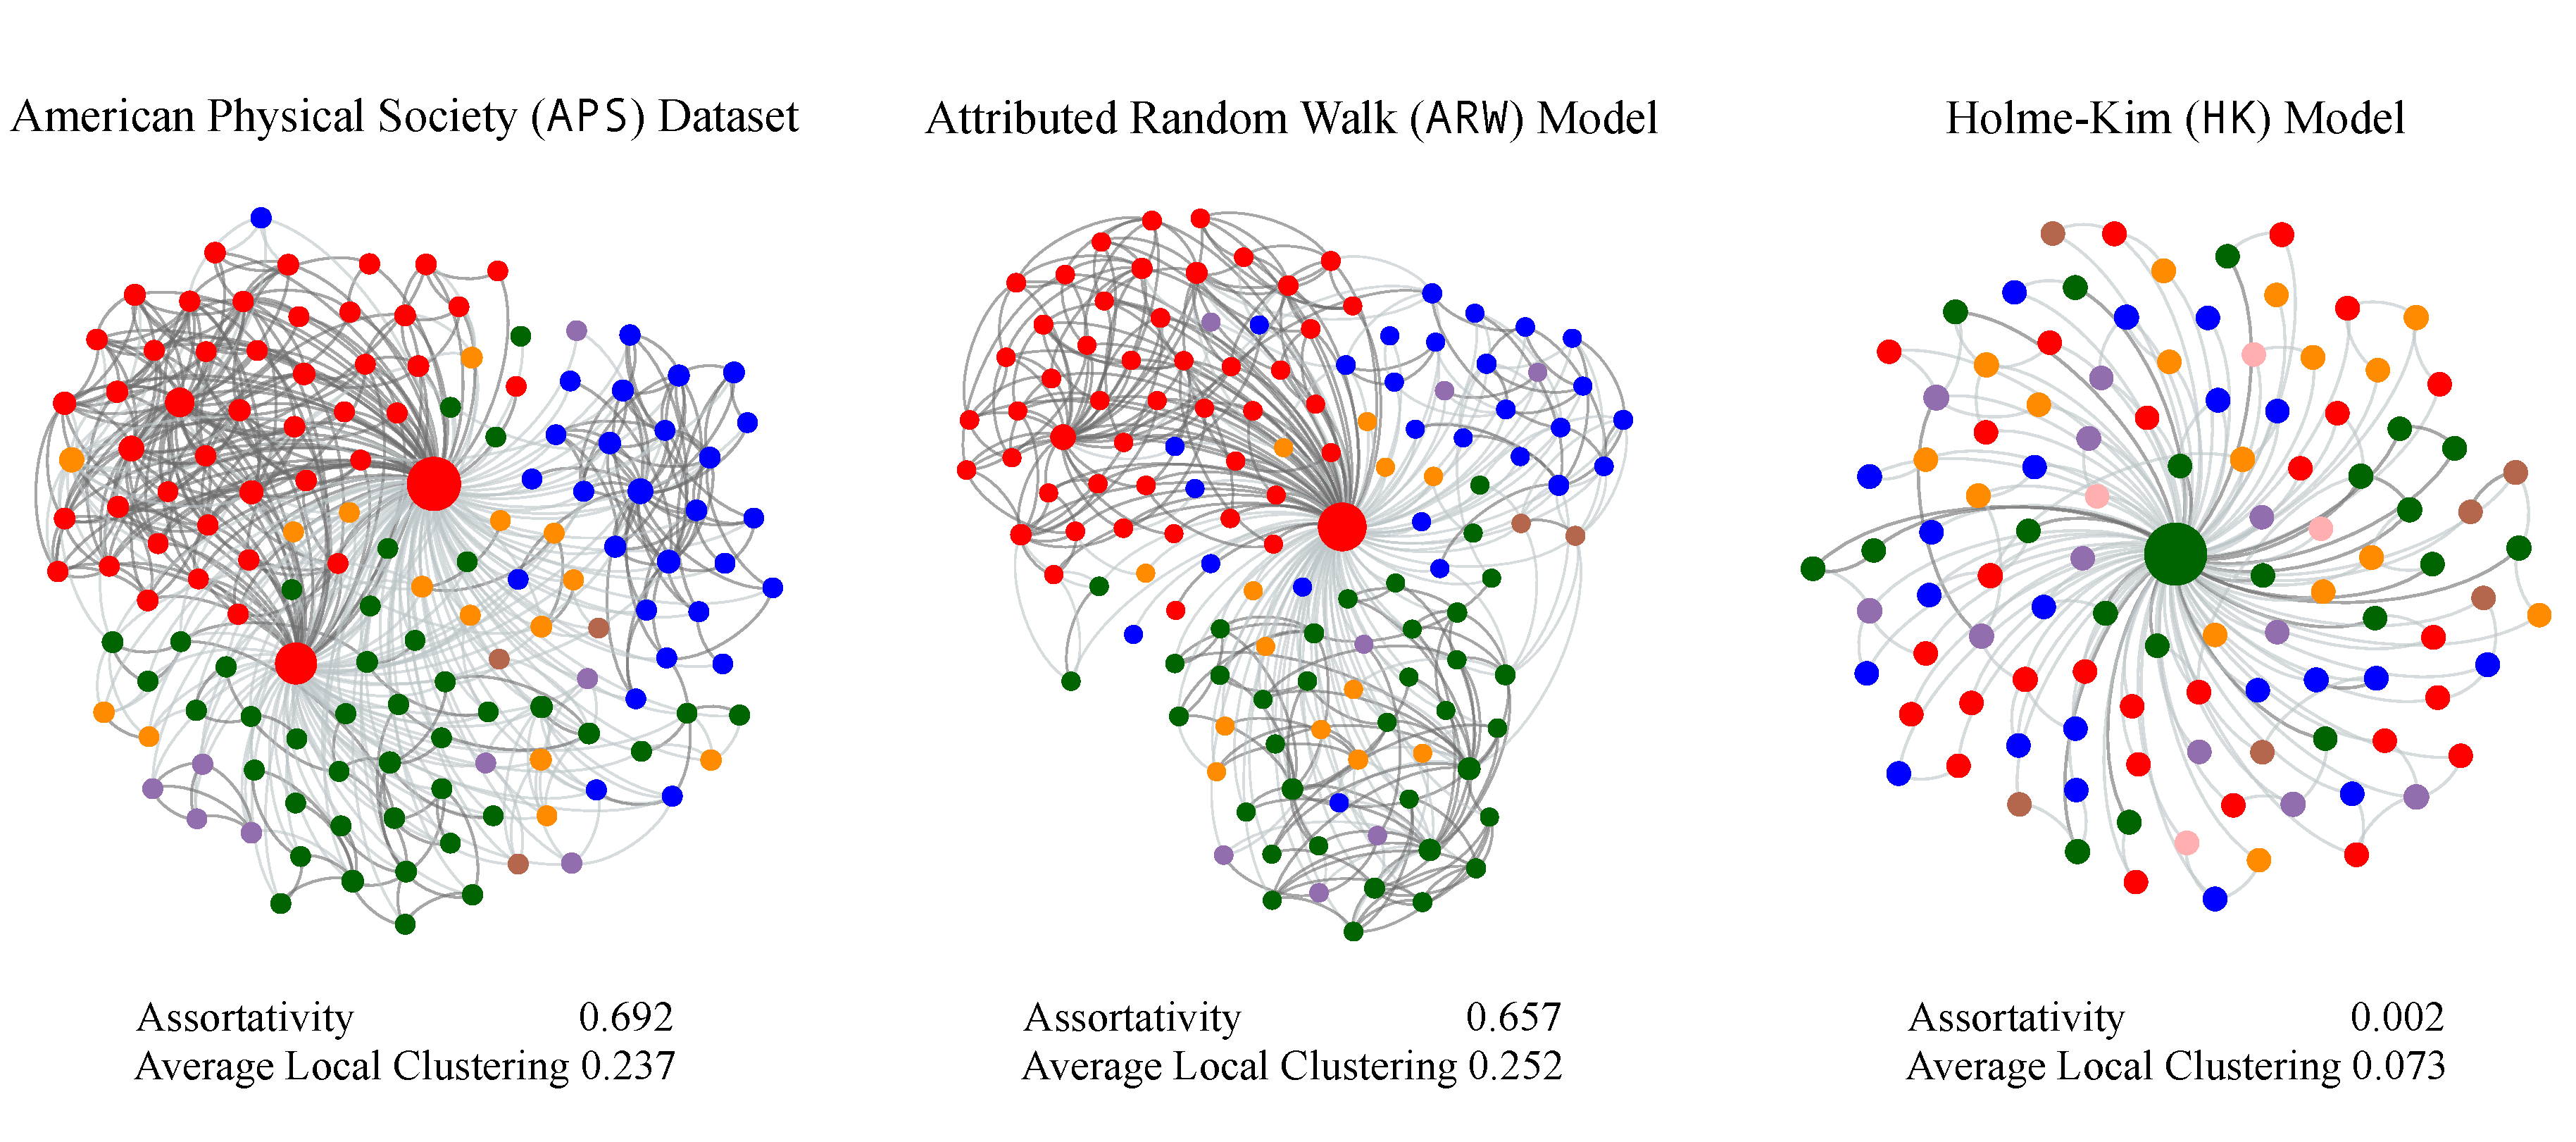
\includegraphics[width=\columnwidth]{intro_plot3}
 \caption{
 }
 \label{fig:intro_plot}
\end{figure}


Our main contributions are as follows:
\begin{itemize}
    \item We propose a model
    of network growth using a local edge formation mechanism that incorporates the
    resource constraints that influence individuals' edge formation mechanisms in
    real-world networks.
    \item We propose a model that jointly explains multiple
    structural properties, including in-degree distribution, clustering, degree
    clustering relationship and edge densification.
\end{itemize}


We conducted extensive experimental results, against state of the art
baselines, on large citation network datasets. We show that our growth model
outperforms that best competing model in jointly and accurately preserving
multiple structural properties---degree distribution, clustering and
degree-clustering relationship---by a significant margin.

The rest of the paper is organized as follows. In~\Cref{sec:Related Work}, we
describe the related work. Then, in~\Cref{sec:Preliminaries}, we define key
structural properties and introduce the datasets. We formally state the goal of
the paper in~\Cref{sec:Problem Statement}. In~\Cref{sec:Empirical Analysis}
and~\Cref{sec:Proposed Model}, we report prominent structural characteristics
of citation networks and propose a network growth model respectively. This is
followed by~\Cref{sec:Experiments}, where we validate our model against
multiple baselines.